\documentclass{standalone}
\usepackage{tikz}
\usetikzlibrary{positioning}

\begin{document}
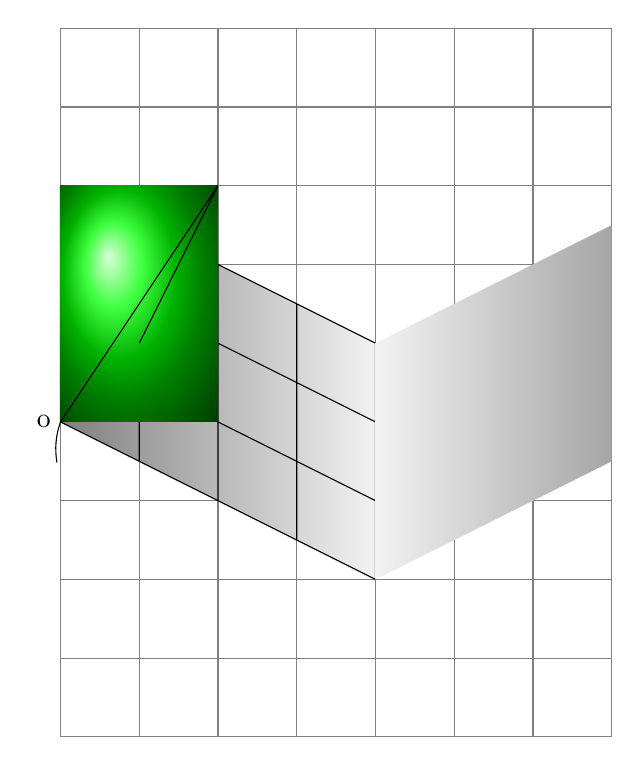
\begin{tikzpicture}
\draw[gray] (0,-4) grid (7,5);
\node[left] at (0,0){o};
 \shade[yslant=-0.5,right color=gray!10, left color=black!50](0,0) rectangle +(4,3);
 \draw[yslant=-0.5] (0,0) grid (4,3);
 \shade[yslant=0.5,right color=gray!70,left color=gray!10]  (4,-4)  rectangle +(3,3);
\draw (0,0) arc (160:190:1);
\shade[ball color=green] (0,0) rectangle (2,3);
\draw(0,0)--+(2,3)--++(1,1);
% \draw[yslant=0.5] (4,-4) grid (7,-1);
%\shade[yslant=0.5,xslant=-1,bottom color=gray!10, top color=black!80] (6,3) rectangle +(-3,-4);
% \draw[yslant=0.5,xslant=-1] (3,-1) grid (6,3);

\end{tikzpicture}
\end{document}
